\section{Background and Design Considerations}
\label{sect:background}
At a cloud cluster node, each instance of a guest operating system runs on a virtual machine, accessing virtual hard disks 
represented as virtual disk image files in the host operating system.
For VM snapshot backup, file-level semantics are normally not provided.
Snapshot operations take place at the virtual device driver level, which
means no fine-grained file system metadata can be used to determine the changed data. 
Backup systems have been developed to use content fingerprints to identify duplicate
content~\cite{venti02,Rhea2008}.  
As discussed earlier, collocating a backup service on the existing
cloud cluster avoids the extra cost to acquire a dedicated backup facility
and reduces the network bandwidth consumption in transferring the
raw data for backup. 
Figure~\ref{fig:collocated} illustrates the cluster architecture where
each physical machine runs a backup service and a distributed file system (DFS)~\cite{googlefs03,hdfs10} 
serves a backup store  for the snapshots.

\begin{figure}[htb]
    \centering
    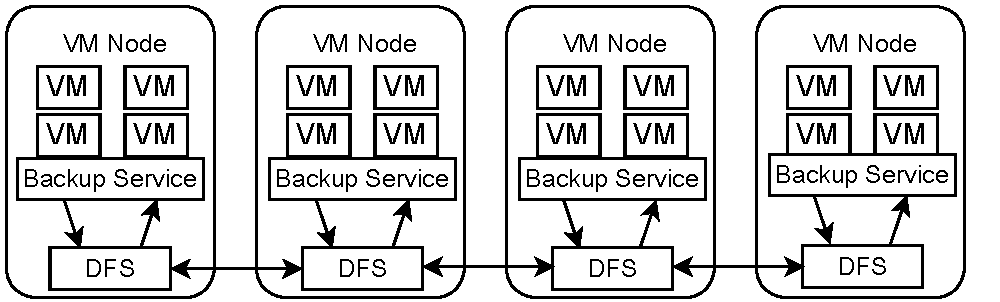
\includegraphics[width=3in]{images/colocated-arch}
    \caption{Collocated VM Backup System.}
    \label{fig:collocated}
\end{figure}

Since it is expensive to compare a large number of chunk signatures for deduplication,
several techniques have been proposed to speedup searching of duplicate
fingerprints. For example, the data domain method ~\cite{bottleneck08} 
uses  an in-memory Bloom filter and a prefetching cache for data chunks  which may be
accessed.  An improvement to this work with parallelization is in ~\cite{MAD210,DEBAR}.
The approximation techniques are studied in~\cite{extreme_binning09,Guo2011,WeiZhangIEEE}  
to reduce memory requirements with the tradeoff of a reduced deduplication ratio.
Additional inline deduplication techniques are studied in ~\cite{sparseindex09,Guo2011,idedup}. 
All of the above approaches have focused on optimization of deduplication
efficiency, and none of them have considered the impact
of deduplication on fault tolerance in the cluster-based environment that we have considered
in this paper.

Our key design consideration is VM dependence minimization during deduplication and file block management.
\begin{itemize}
\item {\em Deduplication localization.}
Because a data chunk is compared with signatures collected from all VMs during
the deduplication process, only one copy of duplicates is stored in the storage,
this artificially creates data dependencies among different VM users. 
Content sharing via deduplication affects fault isolation since machine failures happen periodically 
in a large-scale cloud and
loss of a small number of shared data chunks can 
cause the unavailability of snapshots for a large number of virtual machines.
Localizing the impact of deduplication can increase fault isolation and resilience.
Thus from the fault tolerance point of view,  duplicate sharing among multiple VMs is 
discouraged. 
Another disadvantage of sharing is that it complicates snapshot deletion, 
which  occurs frequently when snapshots expire regularly. 
The mark-sweep approach~\cite{Guo2011} is effective for deletion, and its main cost
is to count if a data chunk is still shared by other snapshots.
Localizing deduplication can  minimize data sharing and simplify deletion while sacrificing 
deduplication efficiency, and  can faciltate parallel execition of snaptshot operations.
\item{\em  Management of file system blocks.}
The file block size in a distributed file system such as  Hadoop and GFS is uniform and large (e.g.  64MB),
 a data chunk in a typical deduplication system is of a nonuniform size with 4KB or 8KB on average.
Packaging data chunks to a file system block can create more data dependence among VMs
since a file block can be shared with even more VMs.
Thus we need to consider a minimum association of a fie system block to VMs in the packaging process.
\end{itemize}

Another consideration is the computing cost of deduplication.
Because of collocation of this snapshot service with other existing cloud services, 
cloud providers will want the backup service to only consume small resources
with a minimal impact to the existing cloud services.
The key resource for signature comparison  is memory for storing the fingerprints. 
We will consider the approximation techniques with less memory consumption along 
with the fault isolation consideration discussed below. 

We call the traditional deduplication approach as   VM-oblivious (VO)
because they compare fingerprints of snapshots without consideration of VM.
With the above  considerations in mind, we study a 
VM-centric approach (called VC)
for a collocated backup service with resource usage friendly
to the existing applications.  
In designing a VC duplication algorithm, we have considered and adopted some of
the following previously-developed techniques.
\begin{itemize}
\item {\bf Version-based change detection}.
VM snapshots can be  backed up  incrementally by identifying file  blocks that have
changed from the previous version of the snapshot~\cite{Clements2009,Vrable2009,TanIPDPS2011}.
Such a scheme  is  VM-centric since deduplication is localized. 
We are seeking for a tradeoff since 
cross-VM  signature comparison can deliver additional compression~\cite{Guo2011,Dong2011,extreme_binning09}.
\item {\bf Stateless  Data Routing}.
One approach for scalable duplicate comparison is to use a content-based hash
partitioning algorithm called stateless data routing~\cite{Dong2011}
that divides the deduplication work with a similarity approximation. This work 
is similar to Extreme Binning\cite{extreme_binning09} and 
each request is routed  to a machine which holds
a Bloom filter  or can fetch on-disk index for additional comparison.
While this approach is VM-oblivious, it motivates us to  use  a combined signature of a dataset to narrow
VM-specific local search.
\item {\bf Sampled Index}.
One effective approach that reduces memory usage is 
to use a sampled index with prefetching, proposed  by Guo and Efstathopoulos\cite{Guo2011}. 
The algorithm is VM oblivious and it is not easy  to adopt for a distributed architecture. 
To use a distributed memory version of the sampled index, every deduplication request
may access a remote machine for index lookup and the overall overhead of latency for all requests
can be significant.  
\end{itemize}

We will first discuss and analyze the integration of the VM-centric deduplication strategies with fault isolation, 
and then present
an architecture and implementation design with deletion support.
